\documentclass[tikz,convert={density=150,size=600,outext=.png}]{standalone}

\begin{document}
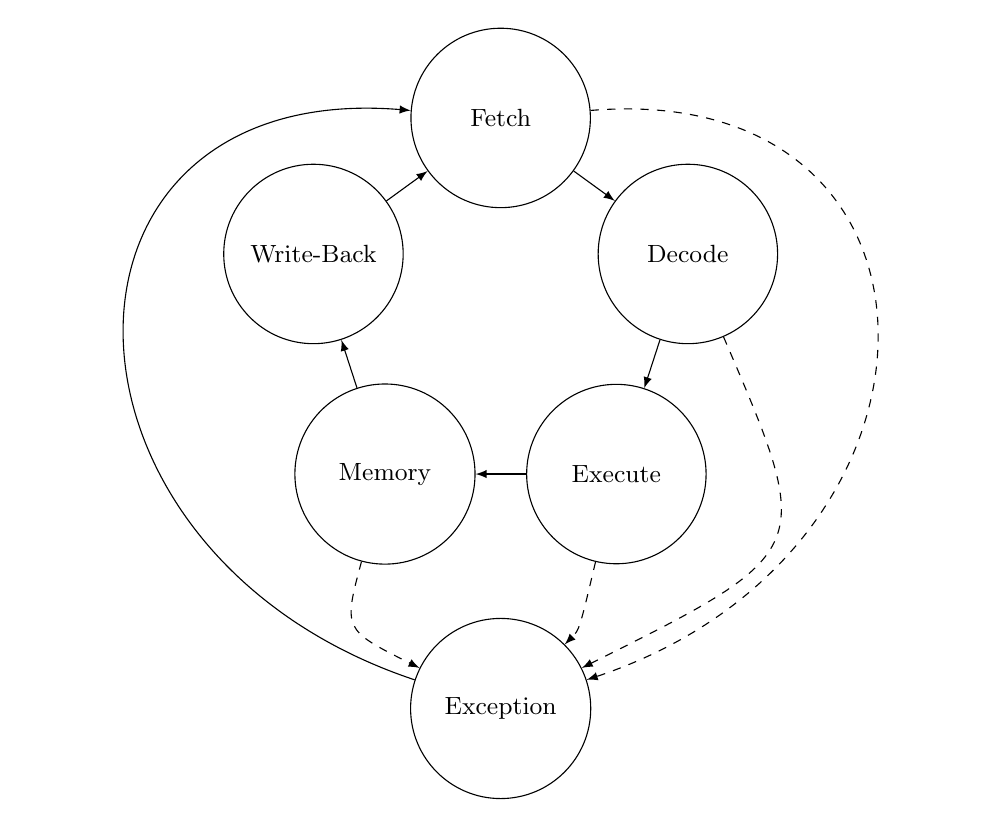
\begin{tikzpicture}[font=\footnotesize, >=latex]
    \foreach \A/\T in { 90/{Fetch},
                        18/{Decode},
                       306/{Execute},
                       234/{Memory},
                       162/{Write-Back}
        } {
        \node[draw, circle, text width = 2cm, text badly centered](stage\A) at (\A:2.5cm) {\small\T};
        }

        \node[draw, circle, text width = 2cm, text badly centered](stageE) at (0,-5.0cm){\small Exception};

        \draw[->] (stage90) -- (stage18);
        \draw[->] (stage18) -- (stage306);
        \draw[->] (stage306) -- (stage234);
        \draw[->] (stage234) -- (stage162);
        \draw[->] (stage162) -- (stage90);

        \draw[dashed, ->] (stage90) .. controls (6,3) and (6,-3) .. (stageE);
        \draw[dashed, ->] (stage18) .. controls (4,-3) .. (stageE);
        \draw[dashed, ->] (stage306) .. controls (1,-4) .. (stageE.north east);
        \draw[dashed, ->] (stage234) .. controls (-2,-4) .. (stageE);

        \draw[->] (stageE) .. controls (-6, -3) and (-6, 3).. (stage90);
\end{tikzpicture}
\end{document}
